% Graphic for TeX using PGF
% Title: /home/robin/Documents/cogradio/doc/thesis/implementation/figures/source.dia
% Creator: Dia v0.97.2
% CreationDate: Wed Jun 10 16:09:56 2015
% For: robin
% \usepackage{tikz}
% The following commands are not supported in PSTricks at present
% We define them conditionally, so when they are implemented,
% this pgf file will use them.
\ifx\du\undefined
  \newlength{\du}
\fi
\setlength{\du}{15\unitlength}
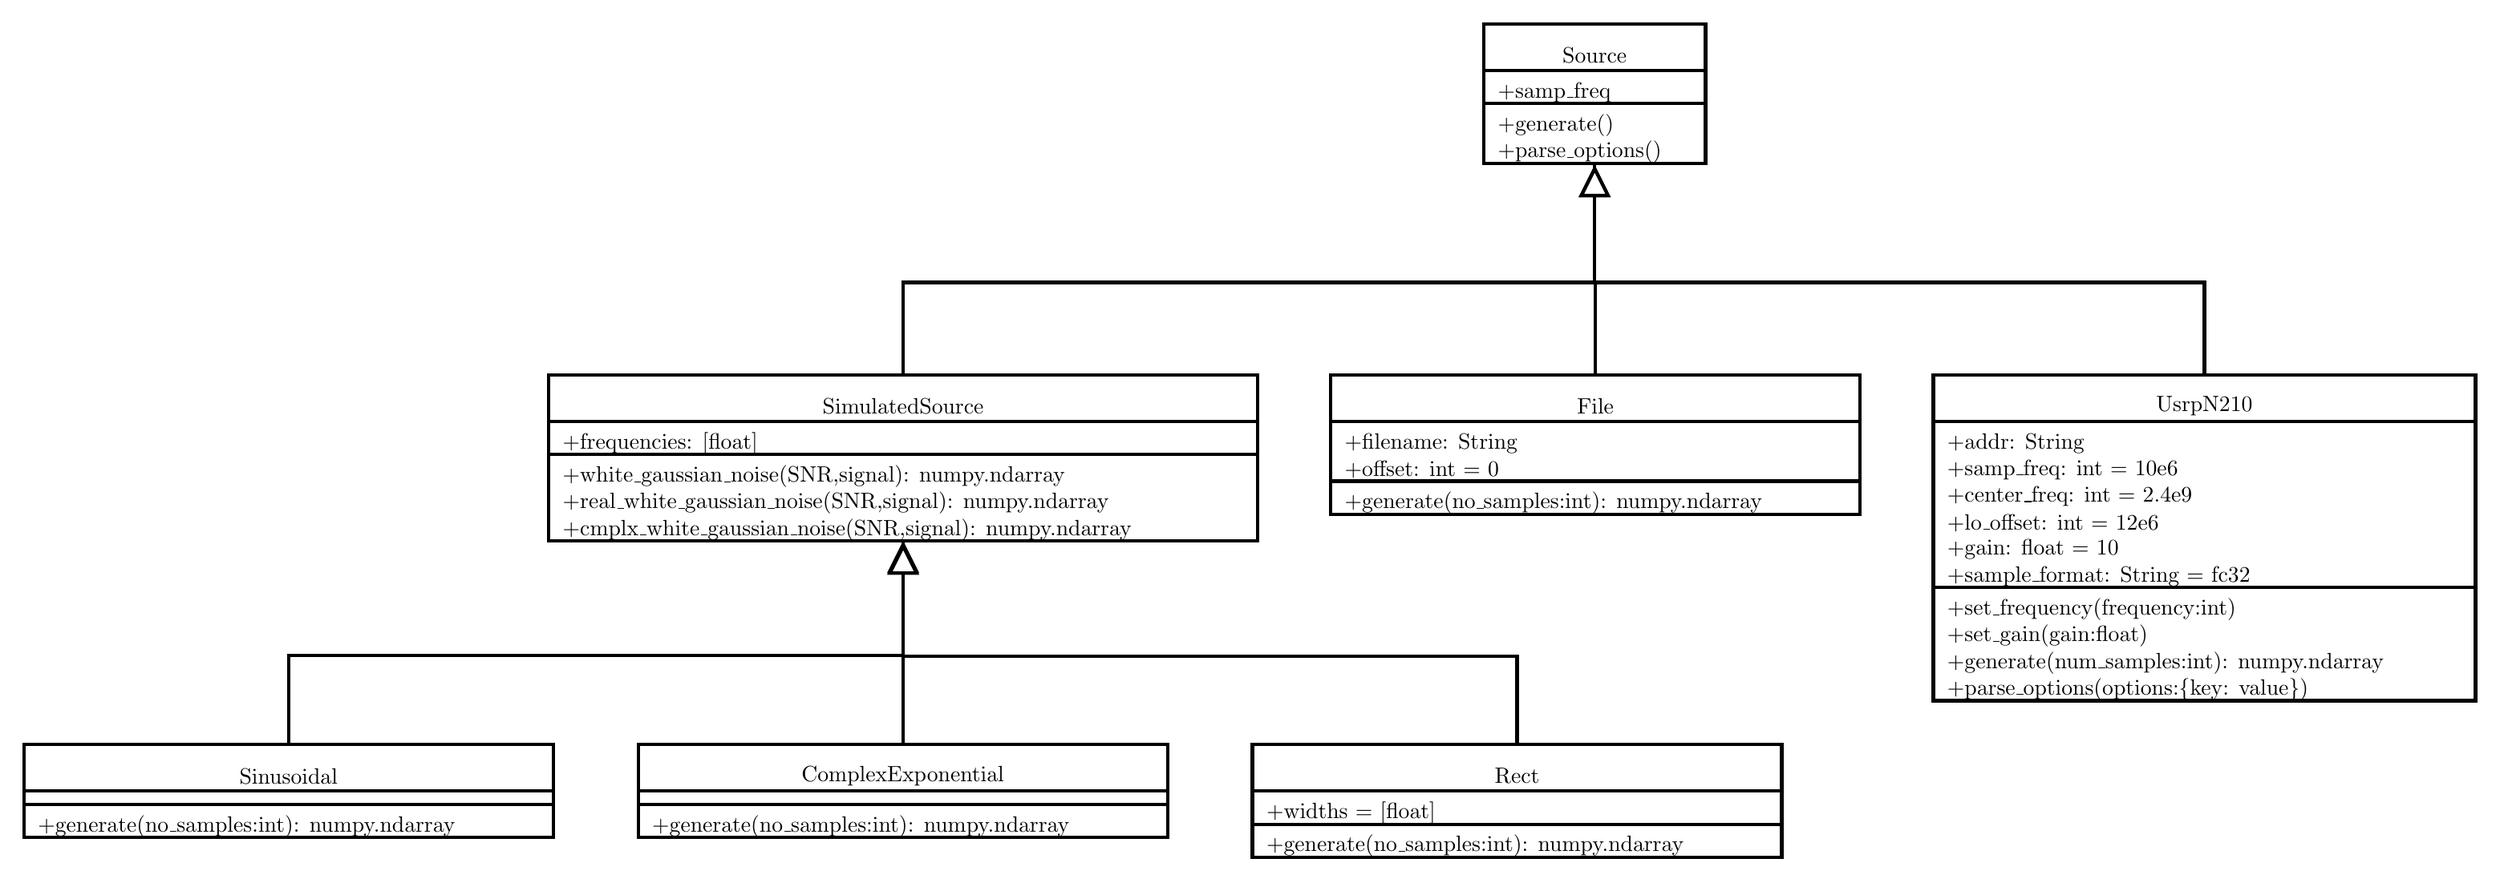
\begin{tikzpicture}
\pgftransformxscale{1.000000}
\pgftransformyscale{-1.000000}
\definecolor{dialinecolor}{rgb}{0.000000, 0.000000, 0.000000}
\pgfsetstrokecolor{dialinecolor}
\definecolor{dialinecolor}{rgb}{1.000000, 1.000000, 1.000000}
\pgfsetfillcolor{dialinecolor}
\pgfsetlinewidth{0.100000\du}
\pgfsetdash{}{0pt}
\definecolor{dialinecolor}{rgb}{1.000000, 1.000000, 1.000000}
\pgfsetfillcolor{dialinecolor}
\fill (28.615000\du,6.737500\du)--(28.615000\du,8.137500\du)--(49.905000\du,8.137500\du)--(49.905000\du,6.737500\du)--cycle;
\definecolor{dialinecolor}{rgb}{0.000000, 0.000000, 0.000000}
\pgfsetstrokecolor{dialinecolor}
\draw (28.615000\du,6.737500\du)--(28.615000\du,8.137500\du)--(49.905000\du,8.137500\du)--(49.905000\du,6.737500\du)--cycle;
% setfont left to latex
\definecolor{dialinecolor}{rgb}{0.000000, 0.000000, 0.000000}
\pgfsetstrokecolor{dialinecolor}
\node at (39.260000\du,7.687500\du){SimulatedSource};
\definecolor{dialinecolor}{rgb}{1.000000, 1.000000, 1.000000}
\pgfsetfillcolor{dialinecolor}
\fill (28.615000\du,8.137500\du)--(28.615000\du,9.137500\du)--(49.905000\du,9.137500\du)--(49.905000\du,8.137500\du)--cycle;
\definecolor{dialinecolor}{rgb}{0.000000, 0.000000, 0.000000}
\pgfsetstrokecolor{dialinecolor}
\draw (28.615000\du,8.137500\du)--(28.615000\du,9.137500\du)--(49.905000\du,9.137500\du)--(49.905000\du,8.137500\du)--cycle;
% setfont left to latex
\definecolor{dialinecolor}{rgb}{0.000000, 0.000000, 0.000000}
\pgfsetstrokecolor{dialinecolor}
\node[anchor=west] at (28.765000\du,8.797500\du){+frequencies: \ensuremath{[}float\ensuremath{]}};
\definecolor{dialinecolor}{rgb}{1.000000, 1.000000, 1.000000}
\pgfsetfillcolor{dialinecolor}
\fill (28.615000\du,9.137500\du)--(28.615000\du,11.737500\du)--(49.905000\du,11.737500\du)--(49.905000\du,9.137500\du)--cycle;
\definecolor{dialinecolor}{rgb}{0.000000, 0.000000, 0.000000}
\pgfsetstrokecolor{dialinecolor}
\draw (28.615000\du,9.137500\du)--(28.615000\du,11.737500\du)--(49.905000\du,11.737500\du)--(49.905000\du,9.137500\du)--cycle;
% setfont left to latex
\definecolor{dialinecolor}{rgb}{0.000000, 0.000000, 0.000000}
\pgfsetstrokecolor{dialinecolor}
\node[anchor=west] at (28.765000\du,9.797500\du){+white\_gaussian\_noise(SNR,signal): numpy.ndarray};
% setfont left to latex
\definecolor{dialinecolor}{rgb}{0.000000, 0.000000, 0.000000}
\pgfsetstrokecolor{dialinecolor}
\node[anchor=west] at (28.765000\du,10.597500\du){+real\_white\_gaussian\_noise(SNR,signal): numpy.ndarray};
% setfont left to latex
\definecolor{dialinecolor}{rgb}{0.000000, 0.000000, 0.000000}
\pgfsetstrokecolor{dialinecolor}
\node[anchor=west] at (28.765000\du,11.397500\du){+cmplx\_white\_gaussian\_noise(SNR,signal): numpy.ndarray};
\pgfsetlinewidth{0.100000\du}
\pgfsetdash{}{0pt}
\definecolor{dialinecolor}{rgb}{1.000000, 1.000000, 1.000000}
\pgfsetfillcolor{dialinecolor}
\fill (12.850000\du,17.850000\du)--(12.850000\du,19.250000\du)--(28.750000\du,19.250000\du)--(28.750000\du,17.850000\du)--cycle;
\definecolor{dialinecolor}{rgb}{0.000000, 0.000000, 0.000000}
\pgfsetstrokecolor{dialinecolor}
\draw (12.850000\du,17.850000\du)--(12.850000\du,19.250000\du)--(28.750000\du,19.250000\du)--(28.750000\du,17.850000\du)--cycle;
% setfont left to latex
\definecolor{dialinecolor}{rgb}{0.000000, 0.000000, 0.000000}
\pgfsetstrokecolor{dialinecolor}
\node at (20.800000\du,18.800000\du){Sinusoidal};
\definecolor{dialinecolor}{rgb}{1.000000, 1.000000, 1.000000}
\pgfsetfillcolor{dialinecolor}
\fill (12.850000\du,19.250000\du)--(12.850000\du,19.650000\du)--(28.750000\du,19.650000\du)--(28.750000\du,19.250000\du)--cycle;
\definecolor{dialinecolor}{rgb}{0.000000, 0.000000, 0.000000}
\pgfsetstrokecolor{dialinecolor}
\draw (12.850000\du,19.250000\du)--(12.850000\du,19.650000\du)--(28.750000\du,19.650000\du)--(28.750000\du,19.250000\du)--cycle;
\definecolor{dialinecolor}{rgb}{1.000000, 1.000000, 1.000000}
\pgfsetfillcolor{dialinecolor}
\fill (12.850000\du,19.650000\du)--(12.850000\du,20.650000\du)--(28.750000\du,20.650000\du)--(28.750000\du,19.650000\du)--cycle;
\definecolor{dialinecolor}{rgb}{0.000000, 0.000000, 0.000000}
\pgfsetstrokecolor{dialinecolor}
\draw (12.850000\du,19.650000\du)--(12.850000\du,20.650000\du)--(28.750000\du,20.650000\du)--(28.750000\du,19.650000\du)--cycle;
% setfont left to latex
\definecolor{dialinecolor}{rgb}{0.000000, 0.000000, 0.000000}
\pgfsetstrokecolor{dialinecolor}
\node[anchor=west] at (13.000000\du,20.310000\du){+generate(no\_samples:int): numpy.ndarray};
\pgfsetlinewidth{0.100000\du}
\pgfsetdash{}{0pt}
\pgfsetmiterjoin
\pgfsetbuttcap
{
\definecolor{dialinecolor}{rgb}{0.000000, 0.000000, 0.000000}
\pgfsetfillcolor{dialinecolor}
% was here!!!
\definecolor{dialinecolor}{rgb}{0.000000, 0.000000, 0.000000}
\pgfsetstrokecolor{dialinecolor}
\draw (39.260000\du,11.737500\du)--(39.260000\du,15.168573\du)--(20.800000\du,15.168573\du)--(20.800000\du,17.799646\du);
}
\definecolor{dialinecolor}{rgb}{0.000000, 0.000000, 0.000000}
\pgfsetstrokecolor{dialinecolor}
\draw (39.260000\du,12.649303\du)--(39.260000\du,15.168573\du)--(20.800000\du,15.168573\du)--(20.800000\du,17.799646\du);
\pgfsetmiterjoin
\definecolor{dialinecolor}{rgb}{1.000000, 1.000000, 1.000000}
\pgfsetfillcolor{dialinecolor}
\fill (39.660000\du,12.649303\du)--(39.260000\du,11.849303\du)--(38.860000\du,12.649303\du)--cycle;
\pgfsetlinewidth{0.100000\du}
\pgfsetdash{}{0pt}
\pgfsetmiterjoin
\definecolor{dialinecolor}{rgb}{0.000000, 0.000000, 0.000000}
\pgfsetstrokecolor{dialinecolor}
\draw (39.660000\du,12.649303\du)--(39.260000\du,11.849303\du)--(38.860000\du,12.649303\du)--cycle;
% setfont left to latex
\pgfsetlinewidth{0.100000\du}
\pgfsetdash{}{0pt}
\definecolor{dialinecolor}{rgb}{1.000000, 1.000000, 1.000000}
\pgfsetfillcolor{dialinecolor}
\fill (31.300000\du,17.850000\du)--(31.300000\du,19.250000\du)--(47.200000\du,19.250000\du)--(47.200000\du,17.850000\du)--cycle;
\definecolor{dialinecolor}{rgb}{0.000000, 0.000000, 0.000000}
\pgfsetstrokecolor{dialinecolor}
\draw (31.300000\du,17.850000\du)--(31.300000\du,19.250000\du)--(47.200000\du,19.250000\du)--(47.200000\du,17.850000\du)--cycle;
% setfont left to latex
\definecolor{dialinecolor}{rgb}{0.000000, 0.000000, 0.000000}
\pgfsetstrokecolor{dialinecolor}
\node at (39.250000\du,18.800000\du){ComplexExponential};
\definecolor{dialinecolor}{rgb}{1.000000, 1.000000, 1.000000}
\pgfsetfillcolor{dialinecolor}
\fill (31.300000\du,19.250000\du)--(31.300000\du,19.650000\du)--(47.200000\du,19.650000\du)--(47.200000\du,19.250000\du)--cycle;
\definecolor{dialinecolor}{rgb}{0.000000, 0.000000, 0.000000}
\pgfsetstrokecolor{dialinecolor}
\draw (31.300000\du,19.250000\du)--(31.300000\du,19.650000\du)--(47.200000\du,19.650000\du)--(47.200000\du,19.250000\du)--cycle;
\definecolor{dialinecolor}{rgb}{1.000000, 1.000000, 1.000000}
\pgfsetfillcolor{dialinecolor}
\fill (31.300000\du,19.650000\du)--(31.300000\du,20.650000\du)--(47.200000\du,20.650000\du)--(47.200000\du,19.650000\du)--cycle;
\definecolor{dialinecolor}{rgb}{0.000000, 0.000000, 0.000000}
\pgfsetstrokecolor{dialinecolor}
\draw (31.300000\du,19.650000\du)--(31.300000\du,20.650000\du)--(47.200000\du,20.650000\du)--(47.200000\du,19.650000\du)--cycle;
% setfont left to latex
\definecolor{dialinecolor}{rgb}{0.000000, 0.000000, 0.000000}
\pgfsetstrokecolor{dialinecolor}
\node[anchor=west] at (31.450000\du,20.310000\du){+generate(no\_samples:int): numpy.ndarray};
\pgfsetlinewidth{0.100000\du}
\pgfsetdash{}{0pt}
\pgfsetmiterjoin
\pgfsetbuttcap
{
\definecolor{dialinecolor}{rgb}{0.000000, 0.000000, 0.000000}
\pgfsetfillcolor{dialinecolor}
% was here!!!
\definecolor{dialinecolor}{rgb}{0.000000, 0.000000, 0.000000}
\pgfsetstrokecolor{dialinecolor}
\draw (39.260000\du,11.737500\du)--(39.260000\du,15.168573\du)--(39.250000\du,15.168573\du)--(39.250000\du,17.799646\du);
}
\definecolor{dialinecolor}{rgb}{0.000000, 0.000000, 0.000000}
\pgfsetstrokecolor{dialinecolor}
\draw (39.260000\du,12.649303\du)--(39.260000\du,15.168573\du)--(39.250000\du,15.168573\du)--(39.250000\du,17.799646\du);
\pgfsetmiterjoin
\definecolor{dialinecolor}{rgb}{1.000000, 1.000000, 1.000000}
\pgfsetfillcolor{dialinecolor}
\fill (39.660000\du,12.649303\du)--(39.260000\du,11.849303\du)--(38.860000\du,12.649303\du)--cycle;
\pgfsetlinewidth{0.100000\du}
\pgfsetdash{}{0pt}
\pgfsetmiterjoin
\definecolor{dialinecolor}{rgb}{0.000000, 0.000000, 0.000000}
\pgfsetstrokecolor{dialinecolor}
\draw (39.660000\du,12.649303\du)--(39.260000\du,11.849303\du)--(38.860000\du,12.649303\du)--cycle;
% setfont left to latex
\pgfsetlinewidth{0.100000\du}
\pgfsetdash{}{0pt}
\definecolor{dialinecolor}{rgb}{1.000000, 1.000000, 1.000000}
\pgfsetfillcolor{dialinecolor}
\fill (49.750000\du,17.850000\du)--(49.750000\du,19.250000\du)--(65.650000\du,19.250000\du)--(65.650000\du,17.850000\du)--cycle;
\definecolor{dialinecolor}{rgb}{0.000000, 0.000000, 0.000000}
\pgfsetstrokecolor{dialinecolor}
\draw (49.750000\du,17.850000\du)--(49.750000\du,19.250000\du)--(65.650000\du,19.250000\du)--(65.650000\du,17.850000\du)--cycle;
% setfont left to latex
\definecolor{dialinecolor}{rgb}{0.000000, 0.000000, 0.000000}
\pgfsetstrokecolor{dialinecolor}
\node at (57.700000\du,18.800000\du){Rect};
\definecolor{dialinecolor}{rgb}{1.000000, 1.000000, 1.000000}
\pgfsetfillcolor{dialinecolor}
\fill (49.750000\du,19.250000\du)--(49.750000\du,20.250000\du)--(65.650000\du,20.250000\du)--(65.650000\du,19.250000\du)--cycle;
\definecolor{dialinecolor}{rgb}{0.000000, 0.000000, 0.000000}
\pgfsetstrokecolor{dialinecolor}
\draw (49.750000\du,19.250000\du)--(49.750000\du,20.250000\du)--(65.650000\du,20.250000\du)--(65.650000\du,19.250000\du)--cycle;
% setfont left to latex
\definecolor{dialinecolor}{rgb}{0.000000, 0.000000, 0.000000}
\pgfsetstrokecolor{dialinecolor}
\node[anchor=west] at (49.900000\du,19.910000\du){+widths = \ensuremath{[}float\ensuremath{]}};
\definecolor{dialinecolor}{rgb}{1.000000, 1.000000, 1.000000}
\pgfsetfillcolor{dialinecolor}
\fill (49.750000\du,20.250000\du)--(49.750000\du,21.250000\du)--(65.650000\du,21.250000\du)--(65.650000\du,20.250000\du)--cycle;
\definecolor{dialinecolor}{rgb}{0.000000, 0.000000, 0.000000}
\pgfsetstrokecolor{dialinecolor}
\draw (49.750000\du,20.250000\du)--(49.750000\du,21.250000\du)--(65.650000\du,21.250000\du)--(65.650000\du,20.250000\du)--cycle;
% setfont left to latex
\definecolor{dialinecolor}{rgb}{0.000000, 0.000000, 0.000000}
\pgfsetstrokecolor{dialinecolor}
\node[anchor=west] at (49.900000\du,20.910000\du){+generate(no\_samples:int): numpy.ndarray};
\pgfsetlinewidth{0.100000\du}
\pgfsetdash{}{0pt}
\pgfsetmiterjoin
\pgfsetbuttcap
{
\definecolor{dialinecolor}{rgb}{0.000000, 0.000000, 0.000000}
\pgfsetfillcolor{dialinecolor}
% was here!!!
\definecolor{dialinecolor}{rgb}{0.000000, 0.000000, 0.000000}
\pgfsetstrokecolor{dialinecolor}
\draw (39.260000\du,11.787811\du)--(39.260000\du,15.193692\du)--(57.700000\du,15.193692\du)--(57.700000\du,17.799573\du);
}
\definecolor{dialinecolor}{rgb}{0.000000, 0.000000, 0.000000}
\pgfsetstrokecolor{dialinecolor}
\draw (39.260000\du,12.699615\du)--(39.260000\du,15.193692\du)--(57.700000\du,15.193692\du)--(57.700000\du,17.799573\du);
\pgfsetmiterjoin
\definecolor{dialinecolor}{rgb}{1.000000, 1.000000, 1.000000}
\pgfsetfillcolor{dialinecolor}
\fill (39.660000\du,12.699615\du)--(39.260000\du,11.899615\du)--(38.860000\du,12.699615\du)--cycle;
\pgfsetlinewidth{0.100000\du}
\pgfsetdash{}{0pt}
\pgfsetmiterjoin
\definecolor{dialinecolor}{rgb}{0.000000, 0.000000, 0.000000}
\pgfsetstrokecolor{dialinecolor}
\draw (39.660000\du,12.699615\du)--(39.260000\du,11.899615\du)--(38.860000\du,12.699615\du)--cycle;
% setfont left to latex
\pgfsetlinewidth{0.100000\du}
\pgfsetdash{}{0pt}
\definecolor{dialinecolor}{rgb}{1.000000, 1.000000, 1.000000}
\pgfsetfillcolor{dialinecolor}
\fill (56.700000\du,-3.812500\du)--(56.700000\du,-2.412500\du)--(63.360000\du,-2.412500\du)--(63.360000\du,-3.812500\du)--cycle;
\definecolor{dialinecolor}{rgb}{0.000000, 0.000000, 0.000000}
\pgfsetstrokecolor{dialinecolor}
\draw (56.700000\du,-3.812500\du)--(56.700000\du,-2.412500\du)--(63.360000\du,-2.412500\du)--(63.360000\du,-3.812500\du)--cycle;
% setfont left to latex
\definecolor{dialinecolor}{rgb}{0.000000, 0.000000, 0.000000}
\pgfsetstrokecolor{dialinecolor}
\node at (60.030000\du,-2.862500\du){Source};
\definecolor{dialinecolor}{rgb}{1.000000, 1.000000, 1.000000}
\pgfsetfillcolor{dialinecolor}
\fill (56.700000\du,-2.412500\du)--(56.700000\du,-1.412500\du)--(63.360000\du,-1.412500\du)--(63.360000\du,-2.412500\du)--cycle;
\definecolor{dialinecolor}{rgb}{0.000000, 0.000000, 0.000000}
\pgfsetstrokecolor{dialinecolor}
\draw (56.700000\du,-2.412500\du)--(56.700000\du,-1.412500\du)--(63.360000\du,-1.412500\du)--(63.360000\du,-2.412500\du)--cycle;
% setfont left to latex
\definecolor{dialinecolor}{rgb}{0.000000, 0.000000, 0.000000}
\pgfsetstrokecolor{dialinecolor}
\node[anchor=west] at (56.850000\du,-1.752500\du){+samp\_freq};
\definecolor{dialinecolor}{rgb}{1.000000, 1.000000, 1.000000}
\pgfsetfillcolor{dialinecolor}
\fill (56.700000\du,-1.412500\du)--(56.700000\du,0.387500\du)--(63.360000\du,0.387500\du)--(63.360000\du,-1.412500\du)--cycle;
\definecolor{dialinecolor}{rgb}{0.000000, 0.000000, 0.000000}
\pgfsetstrokecolor{dialinecolor}
\draw (56.700000\du,-1.412500\du)--(56.700000\du,0.387500\du)--(63.360000\du,0.387500\du)--(63.360000\du,-1.412500\du)--cycle;
% setfont left to latex
\definecolor{dialinecolor}{rgb}{0.000000, 0.000000, 0.000000}
\pgfsetstrokecolor{dialinecolor}
\node[anchor=west] at (56.850000\du,-0.752500\du){+generate()};
% setfont left to latex
\definecolor{dialinecolor}{rgb}{0.000000, 0.000000, 0.000000}
\pgfsetstrokecolor{dialinecolor}
\node[anchor=west] at (56.850000\du,0.047500\du){+parse\_options()};
\pgfsetlinewidth{0.100000\du}
\pgfsetdash{}{0pt}
\definecolor{dialinecolor}{rgb}{1.000000, 1.000000, 1.000000}
\pgfsetfillcolor{dialinecolor}
\fill (52.102500\du,6.737500\du)--(52.102500\du,8.137500\du)--(68.002500\du,8.137500\du)--(68.002500\du,6.737500\du)--cycle;
\definecolor{dialinecolor}{rgb}{0.000000, 0.000000, 0.000000}
\pgfsetstrokecolor{dialinecolor}
\draw (52.102500\du,6.737500\du)--(52.102500\du,8.137500\du)--(68.002500\du,8.137500\du)--(68.002500\du,6.737500\du)--cycle;
% setfont left to latex
\definecolor{dialinecolor}{rgb}{0.000000, 0.000000, 0.000000}
\pgfsetstrokecolor{dialinecolor}
\node at (60.052500\du,7.687500\du){File};
\definecolor{dialinecolor}{rgb}{1.000000, 1.000000, 1.000000}
\pgfsetfillcolor{dialinecolor}
\fill (52.102500\du,8.137500\du)--(52.102500\du,9.937500\du)--(68.002500\du,9.937500\du)--(68.002500\du,8.137500\du)--cycle;
\definecolor{dialinecolor}{rgb}{0.000000, 0.000000, 0.000000}
\pgfsetstrokecolor{dialinecolor}
\draw (52.102500\du,8.137500\du)--(52.102500\du,9.937500\du)--(68.002500\du,9.937500\du)--(68.002500\du,8.137500\du)--cycle;
% setfont left to latex
\definecolor{dialinecolor}{rgb}{0.000000, 0.000000, 0.000000}
\pgfsetstrokecolor{dialinecolor}
\node[anchor=west] at (52.252500\du,8.797500\du){+filename: String};
% setfont left to latex
\definecolor{dialinecolor}{rgb}{0.000000, 0.000000, 0.000000}
\pgfsetstrokecolor{dialinecolor}
\node[anchor=west] at (52.252500\du,9.597500\du){+offset: int = 0};
\definecolor{dialinecolor}{rgb}{1.000000, 1.000000, 1.000000}
\pgfsetfillcolor{dialinecolor}
\fill (52.102500\du,9.937500\du)--(52.102500\du,10.937500\du)--(68.002500\du,10.937500\du)--(68.002500\du,9.937500\du)--cycle;
\definecolor{dialinecolor}{rgb}{0.000000, 0.000000, 0.000000}
\pgfsetstrokecolor{dialinecolor}
\draw (52.102500\du,9.937500\du)--(52.102500\du,10.937500\du)--(68.002500\du,10.937500\du)--(68.002500\du,9.937500\du)--cycle;
% setfont left to latex
\definecolor{dialinecolor}{rgb}{0.000000, 0.000000, 0.000000}
\pgfsetstrokecolor{dialinecolor}
\node[anchor=west] at (52.252500\du,10.597500\du){+generate(no\_samples:int): numpy.ndarray};
\pgfsetlinewidth{0.100000\du}
\pgfsetdash{}{0pt}
\definecolor{dialinecolor}{rgb}{1.000000, 1.000000, 1.000000}
\pgfsetfillcolor{dialinecolor}
\fill (70.200000\du,6.737500\du)--(70.200000\du,8.137500\du)--(86.485000\du,8.137500\du)--(86.485000\du,6.737500\du)--cycle;
\definecolor{dialinecolor}{rgb}{0.000000, 0.000000, 0.000000}
\pgfsetstrokecolor{dialinecolor}
\draw (70.200000\du,6.737500\du)--(70.200000\du,8.137500\du)--(86.485000\du,8.137500\du)--(86.485000\du,6.737500\du)--cycle;
% setfont left to latex
\definecolor{dialinecolor}{rgb}{0.000000, 0.000000, 0.000000}
\pgfsetstrokecolor{dialinecolor}
\node at (78.342500\du,7.687500\du){UsrpN210};
\definecolor{dialinecolor}{rgb}{1.000000, 1.000000, 1.000000}
\pgfsetfillcolor{dialinecolor}
\fill (70.200000\du,8.137500\du)--(70.200000\du,13.137500\du)--(86.485000\du,13.137500\du)--(86.485000\du,8.137500\du)--cycle;
\definecolor{dialinecolor}{rgb}{0.000000, 0.000000, 0.000000}
\pgfsetstrokecolor{dialinecolor}
\draw (70.200000\du,8.137500\du)--(70.200000\du,13.137500\du)--(86.485000\du,13.137500\du)--(86.485000\du,8.137500\du)--cycle;
% setfont left to latex
\definecolor{dialinecolor}{rgb}{0.000000, 0.000000, 0.000000}
\pgfsetstrokecolor{dialinecolor}
\node[anchor=west] at (70.350000\du,8.797500\du){+addr: String};
% setfont left to latex
\definecolor{dialinecolor}{rgb}{0.000000, 0.000000, 0.000000}
\pgfsetstrokecolor{dialinecolor}
\node[anchor=west] at (70.350000\du,9.597500\du){+samp\_freq: int = 10e6};
% setfont left to latex
\definecolor{dialinecolor}{rgb}{0.000000, 0.000000, 0.000000}
\pgfsetstrokecolor{dialinecolor}
\node[anchor=west] at (70.350000\du,10.397500\du){+center\_freq: int = 2.4e9};
% setfont left to latex
\definecolor{dialinecolor}{rgb}{0.000000, 0.000000, 0.000000}
\pgfsetstrokecolor{dialinecolor}
\node[anchor=west] at (70.350000\du,11.197500\du){+lo\_offset: int = 12e6};
% setfont left to latex
\definecolor{dialinecolor}{rgb}{0.000000, 0.000000, 0.000000}
\pgfsetstrokecolor{dialinecolor}
\node[anchor=west] at (70.350000\du,11.997500\du){+gain: float = 10};
% setfont left to latex
\definecolor{dialinecolor}{rgb}{0.000000, 0.000000, 0.000000}
\pgfsetstrokecolor{dialinecolor}
\node[anchor=west] at (70.350000\du,12.797500\du){+sample\_format: String = fc32};
\definecolor{dialinecolor}{rgb}{1.000000, 1.000000, 1.000000}
\pgfsetfillcolor{dialinecolor}
\fill (70.200000\du,13.137500\du)--(70.200000\du,16.537500\du)--(86.485000\du,16.537500\du)--(86.485000\du,13.137500\du)--cycle;
\definecolor{dialinecolor}{rgb}{0.000000, 0.000000, 0.000000}
\pgfsetstrokecolor{dialinecolor}
\draw (70.200000\du,13.137500\du)--(70.200000\du,16.537500\du)--(86.485000\du,16.537500\du)--(86.485000\du,13.137500\du)--cycle;
% setfont left to latex
\definecolor{dialinecolor}{rgb}{0.000000, 0.000000, 0.000000}
\pgfsetstrokecolor{dialinecolor}
\node[anchor=west] at (70.350000\du,13.797500\du){+set\_frequency(frequency:int)};
% setfont left to latex
\definecolor{dialinecolor}{rgb}{0.000000, 0.000000, 0.000000}
\pgfsetstrokecolor{dialinecolor}
\node[anchor=west] at (70.350000\du,14.597500\du){+set\_gain(gain:float)};
% setfont left to latex
\definecolor{dialinecolor}{rgb}{0.000000, 0.000000, 0.000000}
\pgfsetstrokecolor{dialinecolor}
\node[anchor=west] at (70.350000\du,15.397500\du){+generate(num\_samples:int): numpy.ndarray};
% setfont left to latex
\definecolor{dialinecolor}{rgb}{0.000000, 0.000000, 0.000000}
\pgfsetstrokecolor{dialinecolor}
\node[anchor=west] at (70.350000\du,16.197500\du){+parse\_options(options:\{key: value\})};
\pgfsetlinewidth{0.100000\du}
\pgfsetdash{}{0pt}
\pgfsetmiterjoin
\pgfsetbuttcap
{
\definecolor{dialinecolor}{rgb}{0.000000, 0.000000, 0.000000}
\pgfsetfillcolor{dialinecolor}
% was here!!!
\definecolor{dialinecolor}{rgb}{0.000000, 0.000000, 0.000000}
\pgfsetstrokecolor{dialinecolor}
\draw (60.030000\du,0.437762\du)--(60.030000\du,3.962480\du)--(78.342500\du,3.962480\du)--(78.342500\du,6.687198\du);
}
\definecolor{dialinecolor}{rgb}{0.000000, 0.000000, 0.000000}
\pgfsetstrokecolor{dialinecolor}
\draw (60.030000\du,1.349566\du)--(60.030000\du,3.962480\du)--(78.342500\du,3.962480\du)--(78.342500\du,6.687198\du);
\pgfsetmiterjoin
\definecolor{dialinecolor}{rgb}{1.000000, 1.000000, 1.000000}
\pgfsetfillcolor{dialinecolor}
\fill (60.430000\du,1.349566\du)--(60.030000\du,0.549566\du)--(59.630000\du,1.349566\du)--cycle;
\pgfsetlinewidth{0.100000\du}
\pgfsetdash{}{0pt}
\pgfsetmiterjoin
\definecolor{dialinecolor}{rgb}{0.000000, 0.000000, 0.000000}
\pgfsetstrokecolor{dialinecolor}
\draw (60.430000\du,1.349566\du)--(60.030000\du,0.549566\du)--(59.630000\du,1.349566\du)--cycle;
% setfont left to latex
\pgfsetlinewidth{0.100000\du}
\pgfsetdash{}{0pt}
\pgfsetmiterjoin
\pgfsetbuttcap
{
\definecolor{dialinecolor}{rgb}{0.000000, 0.000000, 0.000000}
\pgfsetfillcolor{dialinecolor}
% was here!!!
\definecolor{dialinecolor}{rgb}{0.000000, 0.000000, 0.000000}
\pgfsetstrokecolor{dialinecolor}
\draw (60.030000\du,0.437762\du)--(60.030000\du,3.962500\du)--(60.052500\du,3.962500\du)--(60.052500\du,6.687238\du);
}
\definecolor{dialinecolor}{rgb}{0.000000, 0.000000, 0.000000}
\pgfsetstrokecolor{dialinecolor}
\draw (60.030000\du,1.349566\du)--(60.030000\du,3.962500\du)--(60.052500\du,3.962500\du)--(60.052500\du,6.687238\du);
\pgfsetmiterjoin
\definecolor{dialinecolor}{rgb}{1.000000, 1.000000, 1.000000}
\pgfsetfillcolor{dialinecolor}
\fill (60.430000\du,1.349566\du)--(60.030000\du,0.549566\du)--(59.630000\du,1.349566\du)--cycle;
\pgfsetlinewidth{0.100000\du}
\pgfsetdash{}{0pt}
\pgfsetmiterjoin
\definecolor{dialinecolor}{rgb}{0.000000, 0.000000, 0.000000}
\pgfsetstrokecolor{dialinecolor}
\draw (60.430000\du,1.349566\du)--(60.030000\du,0.549566\du)--(59.630000\du,1.349566\du)--cycle;
% setfont left to latex
\pgfsetlinewidth{0.100000\du}
\pgfsetdash{}{0pt}
\pgfsetmiterjoin
\pgfsetbuttcap
{
\definecolor{dialinecolor}{rgb}{0.000000, 0.000000, 0.000000}
\pgfsetfillcolor{dialinecolor}
% was here!!!
\definecolor{dialinecolor}{rgb}{0.000000, 0.000000, 0.000000}
\pgfsetstrokecolor{dialinecolor}
\draw (60.030000\du,0.437762\du)--(60.030000\du,3.962476\du)--(39.260000\du,3.962476\du)--(39.260000\du,6.687189\du);
}
\definecolor{dialinecolor}{rgb}{0.000000, 0.000000, 0.000000}
\pgfsetstrokecolor{dialinecolor}
\draw (60.030000\du,1.349566\du)--(60.030000\du,3.962476\du)--(39.260000\du,3.962476\du)--(39.260000\du,6.687189\du);
\pgfsetmiterjoin
\definecolor{dialinecolor}{rgb}{1.000000, 1.000000, 1.000000}
\pgfsetfillcolor{dialinecolor}
\fill (60.430000\du,1.349566\du)--(60.030000\du,0.549566\du)--(59.630000\du,1.349566\du)--cycle;
\pgfsetlinewidth{0.100000\du}
\pgfsetdash{}{0pt}
\pgfsetmiterjoin
\definecolor{dialinecolor}{rgb}{0.000000, 0.000000, 0.000000}
\pgfsetstrokecolor{dialinecolor}
\draw (60.430000\du,1.349566\du)--(60.030000\du,0.549566\du)--(59.630000\du,1.349566\du)--cycle;
% setfont left to latex
\end{tikzpicture}
